%\documentclass[aps,showpacs,twocolumn]{revtex4}
\documentclass[aps,preprint]{revtex4}
\newcommand{\dder}{{\rm d}} 
\newcommand{\eexp}{{\rm e}} 
\newcommand{\iima}{{\rm i}} 
\newcommand{\Dt}{{\Delta t}} 
\newcommand{\NT}{{N_{\rm T}}}
\newcommand{\Stild}{\tilde{S}} 
 \newcommand{\Rtild}{{\tilde R}} 
\newcommand{\Itild}{{\tilde I}}


\usepackage{epsfig}
\begin{document}  

\title{The first 100 days:
modeling the evolution of the COVID-19 pandemic
}
\author{Efthimios Kaxiras, Eleni Angelaki, George Neofotistos 
}
\affiliation{Institute for Applied Computational Science, 
Harvard J.A. Paulson School of Engineering 
and Applied Sciences, Harvard University, Cambridge, MA, USA
}

\date{\today}


\begin{abstract}
A simple analytical model for the 2020 COVID-19 pandemic for the first 100 days of the year,
up to April 9, 2020.  The model is based on the popular SIR model for 
describing epidemics, comprising a system of 3 coupled differential equations in an analytical form, which makes it easy to fit data. 
The proposed model contains 3 adjustable parameters which are obtained by fitting actual data 
for 10 countries, a set which includes countries with typical behavior and outliers in the number 
of cases per million of population in each country.  
We analyze these results to infer the physical meaning of the parameters involved. 
We also use the model to make predictions about the total expected number of infections in each country
as well as the date when the number of infections will have reached 99\% of this total. 
\end{abstract}

\maketitle

%\section{Introduction}

The recent pandemic due to the COVID-19 virus has created unprecedented turmoil 
and changed the daily life of people over the entire planet.  It has also yielded 
a grim toll of victims that succumb to its attack. 
While there is great expertise in the medical community and the community of 
statisticians in dealing with epidemics, less is known about this particular disease 
to make reliable predictions for the evolution of the current pandemic. 

In studying past epidemics, scientists have systematically applied “random mixing” models (which assume that an infectious individual may spread the disease to any susceptible member of the population \cite{Kermack_1927}) and contact networks (in which the epidemic spreads only across the edges of a contact network within a population \cite{Barthelemy_2005}, \cite{Ferrari_2006}, \cite{Volz_2008}), Bayesian inference \cite{Groendyke_2011}, models of spatial contacts in large-scale artificial cities \cite{Zhang_2016}, and computational predictions of protein structures \cite{Jumper_2020}, to name just a few of the methodological approaches. 

However, in the case of COVID-19, there is considerable uncertainty in the data collected about infected individuals 
due to the difficulty of testing large numbers of suspected cases. Although a plethora of research studies are currently investigating the COVID-19 epidemiological characteristics (\cite{Sanche_2020}, \cite{Li_2020}, \cite{Imai_2020}, \cite{Rothe_2020}, \cite{Wynants_2020}), it appears that a simple model, which can capture the basic behavior of the 
pandemic phenomenon despite the large uncertainty in the data, can 
hopefully offer some useful guidance for its near-term and longer-term evolution. 
This paper aims to provide such a simple model with very few adjustable parameters.

\section{The model}

\subsection{Derivation of the model}

A simple mathematical description of the spread of an infectious  
disease in a population is the so-called SIR model, 
which divides the (fixed) population of $N$ individuals into three groups:
\begin{itemize}
\item
$S(t)$ the number of individuals susceptible but not yet infected with the disease;
\item
$I(t)$ the number of infected individuals;
\item
$R(t)$ the number of individuals removed (recovered) from the infected group, either by becoming healthy again with long-term immunity or by passing away.
\end{itemize}

The SIR model involves two positive parameters, $\beta$ and $\gamma$ which have the following 
meaning:\\
- $\beta$ describes the effective contact rate of the disease: 
an infected individual comes into contact with $\beta$ other individuals per unit time 
(the fraction that are susceptible to contracting the disease is $S/N$); \\
- $\gamma$ is the mean removal (recovery) rate, that is, $\frac{1}{\gamma}$ is the mean 
period of time during which an infected individual can pass it on before being removed from the group of the infected individuals.\\\\
This model obeys the following differential equations
as first derived by Kermack and McKendrick \cite{Kermack_1927}.

\begin{eqnarray}
\frac{dI}{dt} = \beta I \frac{S}{N} - \gamma I  
\label{eq:SIR_I}
\\
\frac{dS}{dt} = - \beta I \frac{S}{N} 
\label{eq:SIR_S}
\\
\frac{dR}{dt} = \gamma I 
\label{eq:SIR_R}
\end{eqnarray}

This system of equations can be easily solved numerically, as shown in Fig. \ref{fig:FSIR_model}, 
giving the three group populations (S, I, R) as a function of time. 
Kermack and McKendrick pointed out the ``it is impossible from these equations 
to obtain $I(T)$ as an explicit function of $t$'' (p. 713, \cite{Kermack_1927}), 
but provided approximations valid under certain conditions. 
Here we aim to give an approximate analytical solution inspired by the 
numerical simulation.
\begin{figure}[h]
\includegraphics[width=0.52\textwidth]{./figures/FSIR_model.png}
\caption{
\small{
Numerical solution of the SIR model, giving the susceptible $S(t)$ (blue points), 
infected $I(t)$ (orange points)
and removed $R(t)$ (green points) populations as functions of time $t$ in days. 
The parameters of this example are $\beta=0.3$ and $\gamma = 1/10$. 
The corresponding colored lines give the approximate solutions obtained by Eq.s~(\ref{eq:FSIR_S}), 
(\ref{eq:FSIR_R}), (\ref{eq:FSIR_I}). 
}
}
\label{fig:FSIR_model}
\end{figure}

We observe from the numerical solution shown in Fig. \ref{fig:FSIR_model}
that both the susceptible and the removed populations (S and R, respectively) 
behave like sigmoids, which is the typical behavior of solutions to 
differential equations that involve exponential growth and decay. 
Moreover, the infected population is always given by the following expression
\begin{equation}
I(t) = N - S(t) - R(t)
\label{eq:infect-S-R}
\end{equation}
From these observations, we take the approximate solutions to be given by:
\begin{eqnarray}
\Stild & = & N - \frac{N'}{1+\eexp^{-\alpha_1(t-t_1)}} 
\label{eq:FSIR_S}
\\
\Rtild & = & \frac{N'}{1+\eexp^{-\alpha_2(t-t_2)}} 
\label{eq:FSIR_R}
\\
\Itild & = & N - \Stild(t) - \Rtild(t) =  \frac{N'}{1+\eexp^{-\alpha_1(t-t_1)}}
- \frac{N'}{1+\eexp^{-\alpha_2(t-t_2)}} 
\label{eq:FSIR_I}
\end{eqnarray}
where $N'$, $\alpha_1, \alpha_2$, $t_1, t_2$ are treated as adjustable 
parameters (with $t_1$  and $t_2$ representing the temporal midpoint values of the S and the R sigmoid functions of these populations).
In Fig. \ref{fig:FSIR_model} we give an example of how well the 
approximate analytical expressions fit the ``exact'' numerical ones.


\subsection{Analysis of the model}

Here we derive relations between the parameters used in the model of 
Eq.~(\ref{eq:FSIR_S}), (\ref{eq:FSIR_R}), (\ref{eq:FSIR_I}), and the parameters of the original set of differential 
equations, Eq.~(\ref{eq:SIR_I}), (\ref{eq:SIR_S}), (\ref{eq:SIR_R}). 
To keep the expressions simple, we will assume $\alpha_1=\alpha_2=\alpha$ and 
define $\Delta t = t_2 - t_1$. By inserting the expressions for $\Stild$ and $\Itild$ 
in Eq.~(\ref{eq:SIR_S}) we find: 
\begin{equation}
\beta = \alpha  \frac{\eexp^{\alpha(t-t_1)} + \eexp^{\alpha \Delta t}}
{\eexp^{\alpha \Delta t} - 1}
\label{eq:beta}
\end{equation}
Similarly, by inserting the expressions for $\Rtild$ and $\Itild$ in Eq.~(\ref{eq:SIR_R}) we obtain:
\begin{equation}
\gamma = \alpha 
\frac{1+ \eexp^{-\alpha \Delta t} +  \eexp^{\alpha(t-t_2)} +  \eexp^{-\alpha(t-t_2)} \eexp^{-\alpha \Delta t}  }
{4 (1-  \eexp^{-\alpha \Delta t} ) [\cosh(\alpha(t-t_2)/2)]^2}
\label{eq:gamma}
\end{equation}
Thus, in the approximate model described by Eq.~(\ref{eq:FSIR_S}), (\ref{eq:FSIR_R}), (\ref{eq:FSIR_I}), 
the parameters $\beta$ and $\gamma$ of the original SIR model become time-dependent, 
if we treat $\alpha$ as constant to be determined by fitting the data (see next section). 
For this reason, we call this approximate model the ``Forced - SIR'', of FSIR model. 

For $t< t_1$ and assuming that $\alpha \Delta t > 1$ we find that 
$$\beta \approx  \alpha \frac{\eexp^{\alpha \Delta t}}
{\eexp^{\alpha \Delta t} - 1} \approx \alpha,$$
that is, the adjustable parameter of the FSIR model, $\alpha$, is equal, initially, to the (constant) value of the parameter $\beta$ as appears in the original SIR model. Thus, $\beta_{SIR} = \alpha_{FSIR}$.
%It is clear from Eq.~(\ref{eq:beta}) that the FSIR model includes 
%an effective rate $\beta$ which increases with time, since the exponential 
%$\exp[\alpha(t-t_1)]$ in the numerator is a monotonically increasing function of time $t$ 
%and all other terms are constant; this is consistent with the notion of 
%``flattening the curve'', as is commonly referred to 
%the imposition of measures in order to contain the spread of the disease. 
%This consideration suggests that the FSIR model should be well suited 
%to capture the behavior of real data which include this effect. 

It should be mentioned that many recent research studies attempt to model the data of the COVID-19 pandemic 
assuming that the rates $\beta$ and $\gamma$ involved in the original SIR 
model are time-dependent, in order to reflect the imposition of measures designed to slow 
down the spread of the disease. In the FSIR model, $\beta$ and $\gamma$ are time-dependent, but we should not interpret their time-dependence as in the SIR models attempting to model social-distancing measures.

In the FSIR model, the imposition of measures (such as social-distancing and lockdown) is reflected in the value of the adjustable parameter $t_1$ (which is the midpoint of the sigmoid function of the S population); furthermore, the removal (recovery) rate ($\gamma$) corresponds to $\frac {1}{\Delta t}$ as will be explained below. Therefore, as they are adjustable parameters, there is no need to impose time-dependent conditions on them.

%If we use a Taylor expansion of the exponential in $\Delta t$ in the Eq.~(\ref{eq:gamma}) and 
%keep the lowest order terms as appropriate, we find:
$$\gamma \approx \frac{1}{\Delta t}, \; \; {\rm for} \; \; \alpha \Delta t \ll 1,$$
showing that $\Delta t$ is closely related to the value of $\gamma$ in the SIR model. 
However, this condition does not hold for the data we consider below, as the FSIR estimated values
of the parameters are $\alpha=0.25$ and $\Delta t \approx 20$, 
giving $\alpha \Delta t \approx 5$. Nevertheless, the FSIR estimated value of $\alpha \Delta t \approx 5$ (which represents the basic reproduction number $R_0$ of the FSIR model) is in excellent agreement with recently reported median value of 5.7 (95\% CI 3.8–8.9) of the basic reproduction number $R_0$ of the COVID-19 pandemic \cite{Sanche_2020}. Therefore, we will keep considering $\frac {1}{\Delta t}$ as the removal (recovery) rate in the FSIR model.  
 

\section{Application to 10 countries}

We use our approximate analytical solutions to fit the behavior of 
infected populations of 10 countries, as obtained from \cite{ECDC_source}, 
for a period of 100 days ending on April 8, 2020.  
The choice of the countries aims to capture extreme cases as well as 
typical cases.  This is explained in Fig. \ref{fig:daily_10}.

\begin{figure}[h]
\hspace{-0.04\textwidth}
\includegraphics[width=0.52\textwidth]{./figures/Total_10.png}
\hspace{-0.04\textwidth}
\includegraphics[width=0.52\textwidth]{./figures/Total_scale_10.png}
\caption{
\small{
Daily reports of infected individuals in 10 countries. 
{\bf Left:} the raw data as reported in \cite{ECDC_source};
the outliers are Greece (GRC, blue line) with the lowest number of cases, 
and the United States (USA, purple line) with the highest number of cases. 
{\bf Right}: the data scaled by the population of each country
(which is tabulated in the same source);
in the scaled data, it is clear that China (CHN, red line) and Greece (GRC, blue line) 
are outliers as having very low number of infections, while Spain (ESP, red line) 
and Switzerland (CHE, grey line) and the United States (USA, purple line) 
are outliers as having the largest 
number of infections, in descending order.  
All sets represent cases per million of the population of the 
respective country. 
}
}
\label{fig:daily_10}
\end{figure}

In order to obtain a meaningful fit, we had to consider data that show a 
monotonic increase at the beginning.  This means that a few data points in 
each case were excluded, as they corresponded to sporadic reports 
of very few cases (typically 1 to 10 in a given day, interspersed by several days 
of 0 cases).  In practice this means that the fitting begins at a certain 
cutoff day denoted as $t_0$. 
Also, for simplicity we use the approximation $N' = N$ in 
Eq.~(\ref{eq:FSIR_S}), (\ref{eq:FSIR_R}), (\ref{eq:FSIR_I}), which 
is a reasonable approximation. Finally, to make the fit more robust 
and simpler, we chose $\alpha_1=\alpha_2=\alpha$. 
Moreover, we found by trial-and-error that the value $\alpha=0.25$ is 
the optimal choice for all the countries we considered.  
This  leaves three adjustable parameters in the model that 
can be varied to obtain the best fit to the data, namely $t_1$, $t_2$ and $N'$; 
instead of $t_1$ and $t_2$, we elected to use instead as independent 
parameters $t_1$ and $\Delta t = t_2-t_1$. 
The best fit here is defined in the Root-Mean-Square (RMS) sense. 
To have a measure of the fit that is comparable between different 
countries, we defined the ``quality of fit'' as:
\begin{equation}
Q_{\rm fit} = \frac{1}{N'} {\rm RMSE}
\label{eq:quality_fit}
\end{equation}
which is expressed as a percentage (multiplied by a factor of 100). 
The resulting values of the parameters, including our choices of $t_0$, 
are given in Table \ref{table:parameters}.

\begin{figure}[h]
\hspace{-0.04\textwidth}
\includegraphics[width=0.52\textwidth]{./figures/Daily_CHN.png}
\hspace{-0.04\textwidth}
\includegraphics[width=0.52\textwidth]{./figures/Total_CHN.png}

\hspace{-0.04\textwidth}
\includegraphics[width=0.52\textwidth]{./figures/Daily_GRC.png}
\hspace{-0.04\textwidth}
\includegraphics[width=0.52\textwidth]{./figures/Total_GRC.png}


\hspace{-0.04\textwidth}
\includegraphics[width=0.52\textwidth]{./figures/Daily_ESP.png}
\hspace{-0.04\textwidth}
\includegraphics[width=0.52\textwidth]{./figures/Total_ESP.png}


\hspace{-0.04\textwidth}
\includegraphics[width=0.52\textwidth]{./figures/Daily_USA.png}
\hspace{-0.04\textwidth}
\includegraphics[width=0.52\textwidth]{./figures/Total_USA.png}
\caption{
\small{
Data for China (CHN), Greece (GRC), Spain (ESP) and the United States of America (USA).
Red dots are the daily data reported in Ref. \cite{ECDC_source}, the green lines are the fits 
by the model.
}
}
\label{fig:data_outliers}
\end{figure}
In Fig. \ref{fig:data_outliers} we give some examples of the actual fits for the  
outliers countries (China, Greece, USA and Spain). 

\begin{table}
\begin{center}
\begin{tabular}{| c |l r | r | r | r | r | r | r | r|}\hline
Index & Country & (Symbol) &  $\; \; \; \; t_0 $  & $\; \; t_1$ & $\Dt$ & $N'$  & $Q_{\rm fit}$ & $\NT$ &  $D$ \\ 
 &  &  & (days)  & (days) & (days) &  & (\%) &  & (days) \\  \hline 
0 & China & (CHN) & 18 & 18.5 & 11.1 & 7,344 & 17.91 & 81,100 & $-40$ \\
1 & Greece & (GRC) & 61 & 17.2 & 25.4 & 86 & 25.40 & 2,200 & 12 \\
2 & Italy & (ITA) & 54 & 21.3 & 25.8 & 5,970 & 8.15 & 153,900 & 10 \\
3 & Switzerland & (CHE) & 57 & 22.4 & 19.1 & 1,330 & 11.98 & 25,400  & 10 \\
4 & Netherlands & (NLD) & 60 & 23.2 & 21.7 & 1,212 & 7.15 & 26,300 & 14 \\
5 & Germany & (DEU) & 58 & 24.2 & 21.7 & 6,225 & 13.29 & 135,000 & 13 \\
6 & France & (FRA) & 58 & 26.5 & 18.2 & 5,401 & 14.70 & 98,400 & 13 \\
7 & Spain & (ESP) & 56 & 27.2 & 16.1 & 10,539 & 6.42 & 169,700 & 11\\
8 & United Kingdom & (GBR) & 60 & 29.9 & [24] & 5,054 & 8.01 & [121,000] & [22] \\
9 & United States & (USA) & 60 & 28.7 & [24] & 33,750 & 4.61 & [808,700] & [21] \\
\hline
\end{tabular}
\caption{
\label{table:parameters}
\small{
The values of the various parameters that enter in the FSIR model of Eq.~(\ref{eq:FSIR_S}), 
(\ref{eq:FSIR_R}), (\ref{eq:FSIR_I}), for the 10 countries considered (see text 
for details). The next-to-last column includes the values for the {\em expected} total number 
of cases $N_T$ when the number of infections has dropped to near zero, and is an 
{\em extrapolated} value (rounded to the nearest 100).  The last column includes 
the number of days $D$ until the value of $N_T$ has reached 99\% of its final value;
a negative number (for China) indicates that this date has already passed.  Numbers in 
square brackets are {\em not} the result of fitting, but represent reasonable  estimates (see text). 
}}
\end{center}
\end{table}

The values of the parameters obtained reveal interesting behavior.
\begin{itemize}
\item{$t_0$: 
The value of this parameter is very similar for all countries, except for China
with $t_0 = 18$. 
This simply reflects the fact that the pandemic originated in China and then 
spread through the rest of the world. The rest of the countries have starting dates 
of the exponential increase within one week from the earliest, Italy (with $t_0 = 54$)
to the latest, Greece (with $t_0 = 61$).
The time lag between most countries and China is approximately 42 days or 6 weeks. 
}
\item{$t_1$: 
This value indicates the position of the mid-point of the sigmoid that 
represents the behavior of the susceptible population. 
The shorter it is, the sooner the country attempted to introduce measures 
to limit the spread of the disease.  The two countries with the shortest $t_1$ values 
are China and Greece; unsurprisingly, these two countries also have the lowest 
number of cases per million, as already shown in Fig. \ref{fig:daily_10}. 
We will also see that these two countries have the lowest expected {\em total} number
of cases per million. 
}
\item{$\Delta t$: 
This value indicates the lag between the sigmoid that describes the recovered 
population and the sigmoid of the susceptible population. We showed earlier 
that this value is related to the effective rate of recovery, $\gamma$, of the SIR model, 
that is, $\gamma \approx \frac {1}{\Delta t}$, in a certain limit. 
For most countries $\Delta t$ is close to 20 days ($\sim 3$ weeks), a value consistent with an estimated median time of approximately 2 weeks from onset to clinical recovery for mild cases, and 3-6 weeks for patients with severe or critical disease \cite{WHO_China_2020}. China shows an unusual lower value, $\Delta t$=11.0.
This value is Using available preliminary data, the median time from onset to clinical recovery for mild cases is approximately 2 weeks and is 3-6 weeks for patients with severe or critical disease
We note that in order to obtain the value of this parameter, the curve of the 
daily values of $\Itild$ has to have passed its maximum value, otherwise the 
fit is not sensitive to this parameter and produces unphysical values.  
For example, in the case of USA, which 
clearly has not reached the maximum yet, the fit does not yield a meaningful value for 
$\Delta t$; instead, we used a value that does not affect the quality of the fit 
to more that the second significant digit of $Q_{\rm fit}$ and is 
quite close to the average for the other countries. The value of this parameter 
has a significant effect on the total expected number of cases (see below). 
}
\item{$N'$: the value of this parameter is representative of the number of daily cases 
near the peak of the $\Itild$ curve. It is close to reported values for this quantity for 
all the countries. 
}
\end{itemize}

In Table \ref{table:parameters} we also include the values for the quality of the fit, 
which range from 4.6 (USA) to 25 (Greece), representing a measure of the 
relative noise in the data.  The noise is largest for Greece because the numbers are 
rather small, and smallest for the USA because the numbers are quite large. 


Using the analytic expression for $\Itild(t)$ we can extrapolate to long times and 
try to obtain an estimate for the total value of cases over a long period, 
when the number of daily cases of infection have essentially dropped to 
negligible levels (this corresponds to $\Itild(t) \approx 0$).  
We call this asymptotic value $N_T$ and report it in Table \ref{table:parameters}.  We caution that, 
as with any extrapolation, this number should viewed with great caution. 
For instance, in the case of USA, the choice of the value for $\Delta t$ that 
we have chosen significantly affects this quantity: our best estimate of
$\Delta t$ is 24; changing this value to 22 (a change of about $-10$\%) 
reduces the value of $N_T$ to $ \approx 742,000$ (a change of about $-8$\%). 
Similar comments apply to the case of UK, which has also not reached the peak.
Our best estimate for $\Delta t$ in this case is 24; changing this value to 22 
(a change of about $-10$\%) reduces the value of $N_T$ 
to $\approx 111,000$ (a change of about $-8$\%).


It is interesting to speculate on the meaning of these results. In Fig. \ref{fig:t1_Nt_10} 
we provide a visualization of the values of $t_1$ and $N_T$, normalized by 
the population of each country so that the values shown are per million of population. 
Clearly, a low value of $t_1$ is correlated to a low $N_T$, as the examples 
of China and Greece demonstrate.  In other words, early adoption of measures to 
contain the spread of the disease pay off.  
It is not clear why Italy (ITA) and Switzerland (CHE) do not follow this pattern. 
On the other extreme, the countries with high values of $t_1$ also have high values 
of $N_T$, especially Spain (ESP) and the USA.  
In the case of the UK, which has the highest $t_1$ value, the value of $N_T$ is not 
exceptionally high.
We emphasize again here the caution with which $N_T$ should be 
viewed, being an extrapolated quantity. 

\begin{figure}[h]
\hspace{-0.04\textwidth}
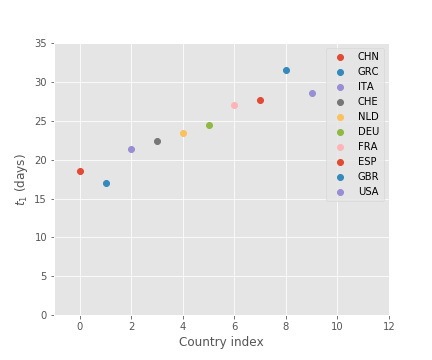
\includegraphics[width=0.52\textwidth]{./figures/t1_10.png}
\hspace{-0.04\textwidth}
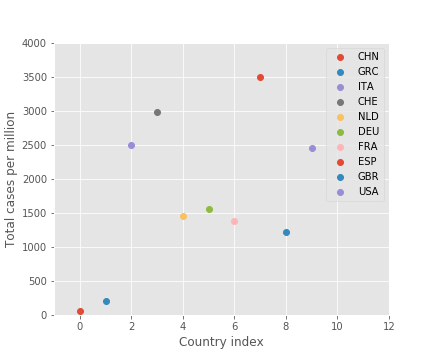
\includegraphics[width=0.52\textwidth]{./figures/Nt_10.png}
\caption{
\small{
Visualization of the values of the parameter $t_1$ and the expected 
total number of cases $N_T$ for 10 countries. 
The values of $N_T$ have been scaled by the population of each country,
so they are expressed per million of population. 
}
}
\label{fig:t1_Nt_1 0}
\end{figure}


\begin{thebibliography}{99}

\bibitem{Kermack_1927}
W. O. Kermack and A. G. McKendrick, "A contribution to the mathematical theory of epidemics",  Proc. Roy. Soc. A, {\bf 115}, 772 (1927).

\bibitem{Barthelemy_2005}
M. Barthélemy, A. Barrat, R. Pastor-Satorras, A. Vespignani, "Dynamical patterns of epidemic outbreaks in complex heterogeneous networks", J Theor Biol. 2005;235(2):275–288. doi:10.1016/j.jtbi.2005.01.011

\bibitem{Ferrari_2006}
M. J. Ferrari, S. Bansal, L. A. Meyers, O. N. Bjørnstad, "Network frailty and the geometry of herd immunity", Proc Biol Sci. 2006;273(1602):2743–2748. doi:10.1098/rspb.2006.3636

\bibitem{Volz_2008}
E. Volz, "SIR dynamics in random networks with heterogeneous connectivity", J Math Biol. 2008 Mar;56(3):293-310. doi: 10.1007/s00285-007-0116-4.  

\bibitem{Groendyke_2011}
C. Groendyke, D. Welch, and D. R. Hunter, "Bayesian Inference for Contact Networks Given Epidemic Data", Scandinavian Journal of Statistics,
Vol. 38, No. 3 (September 2011), pp. 600-616.

\bibitem{Zhang_2016}
M. Zhang, A. Verbraeck, R. Meng, B. Chen, and X. Qiu, (2016) "Modeling Spatial Contacts for Epidemic Prediction in a Large-Scale Artificial City" Journal of Artificial Societies and Social Simulation 19 (4) 3 (downloaded from http://jasss.soc.surrey.ac.uk/19/4/3.html on 4/9/2020). doi: 10.18564/jasss.3148.
-616.

\bibitem{Jumper_2020}
J. Jumper, K. Tunyasuvunakool, P. Kohli, D. Hassabis, and the AlphaFold Team, "Computational predictions of protein structures associated with COVID-19", Version 2, DeepMind website, 8 April 2020, https://deepmind.com/research/open-source/computational-predictions-of-protein-structures-associated-with-COVID-19.

\bibitem{Sanche_2020}
S. Sanche, Y. T. Lin, C. Xu, E. Romero-Severson, N. Hengartner, R. Ke, "High contagiousness and rapid spread of severe acute respiratory syndrome coronavirus 2" . Emerg Infect Dis. 2020 Jul [date cited]. https://doi.org/10.3201/eid2607.200282. DOI: 10.3201/eid2607.200282

\bibitem{Li_2020}
Q. Li , X. Guan, P. Wu, X. Wang, L. Zhou, Y. Tong, et al., "Early transmission dynamics in Wuhan, China, of novel coronavirus-infected pneumonia", N Engl J Med. 2020;382:1199–207. 

\bibitem{Imai_2020}
N. Imai, I. Dorigatti, A. Cori, S. Riley, N. M. Ferguson, "Estimating the potential total number of novel coronavirus cases in Wuhan City, China" [cited 2020 Feb 2]. https://www.imperial.ac.uk/media/imperial-college/medicine/sph/ide/gida-fellowships/2019-nCoV-outbreak-report-17-01-2020

\bibitem{Rothe_2020}
C. Rothe, M. Schunk, P. Sothmann, G. Bretzel, G. Froeschl, C. Wallrauch, et al., "Transmission of 2019-nCoV infection from an asymptomatic contact in Germany",  N Engl J Med. 2020;382:970–1.

\bibitem{Wynants_2020}
L. Wynants, B. Van Calster Ben, M. Bonten, G. Collins, T. Debray, M. De Vos et al., "Prediction models for diagnosis and prognosis of covid-19 infection: systematic review and critical appraisal" BMJ 2020; 369 :m1328

\bibitem{ECDC_source}
https://opendata.ecdc.europa.eu/covid19/casedistribution/csv

\bibitem{WHO_China_2020}
Report of the WHO-China Joint Mission on Coronavirus Disease 2019 (COVID-19) 16-24 February 2020
https://www.who.int/docs/default-source/coronaviruse/who-china-joint-mission-on-covid-19-final-report.pdf




\end{thebibliography}

\end{document}
